% ОБЯЗАТЕЛЬНО ИМЕННО ТАКОЙ documentclass!
% (Основной кегль = 14pt, поэтому необходим extsizes)
% Формат, разумеется, А4
% article потому что стандарт не подразумевает разделов
% Глава = section, Параграф = subsection
% (понятия "глава" и "параграф" из документа, описывающего диплом)
\documentclass[a4paper,article,14pt]{extarticle}

% Подключаем главный пакет со всем необходимым
\usepackage{spbudiploma_tempora}

% Пакеты по желанию (самые распространенные)
% Хитрые мат. символы
\usepackage{euscript}
% Таблицы
\usepackage{longtable}
\usepackage{makecell}
% Картинки (можно встявлять даже pdf)
\PassOptionsToPackage{pdftex}{graphicx}
\usepackage{adjustbox}

\usepackage{amsthm,amssymb, amsmath}
\usepackage{textcomp}


\begin{document}

% Титульник в файле titlepage.tex
\input{parts/titlepage.tex}

% Содержание
\tableofcontents
\pagebreak

\specialsection{Введение}

\specialsubsection{Актуальность работы}
В настоящее время разработка компьютерных игр (\textit{геймдев}, \textit{gamedev}) является быстроразвивающейся индустрией. При этом научные исследования последних лет показывают, что методологии и достижения в разработке компьютерных игр находят применение не только в сфере развлечений, но и в:
\begin{itemize}
	\item[--] медицине (терапия расстройств аутистического спектра (РАС), детского церебрального паралича (ДЦП)) \cite{lopes2018games,hassan2021serious};
	\item[--] образовании (обучение программированию и другим дисциплинам) \cite{vahldick2020blocks,mayer2019computer};
	\item[--] бизнесе (геймификация корпоративных систем) \cite{augustin2016we}.
\end{itemize}

При разработке игр команды нередко сталкиваются с рядом глобальных проблем. К ним можно отнести как технические ошибки (недостаточная оптимизация, баги), так и ошибки в дизайне (неясное видение дизайна игры, отсутствие <<фактора удовольствия>>) \cite{politowski2021game}.

Все большее количество проблем исследователи пытаются разрешить с помощью использования искусственного интеллекта. Основными сферами применения ИИ являются создание правдоподобных неигровых персонажей (\textit{non-playable character}, \textit{NPC}), процедурная генерация контента, моделирование опыта игроков, помощь с геймдизайном \cite{xia2020recent}.

Одним из факторов возникновения проблем является ручное тестирование, превалирующее в разработке видеоигр \cite{santos2018computer}, которое не всегда позволяет выявить возможные ошибки. Оно полностью полагается на \textit{ad-hoc} мышление игровых тестировщиков, играющих в одну и ту же игру снова и снова. Все чаще игры выходят с ошибками, которые разработчики вынуждены исправлять в последующих обновлениях \cite{truelove2021we}. В этой связи актуальной задачей является автоматизирование тестирования игрового процесса, отличающегося от <<традиционного>> процесса разработки ПО и слабо поддающегося устоявшимся методам автоматизации \cite{politowski2021game,murphy2014cowboys}. Частичная или полная автоматизация позволила бы специалистам сконцентрироваться на других особенностях игр, таких как баланс, логика и фактор удовольствия.

Перспективным инструментом автоматизации является обучение с подкреплением (\textit{reinforcement learning}, \textit{RL}) на основе нейронных сетей. RL успешно показывает себя в хорошо понимаемых, воспроизводимых процессах. Кроме того, алгоритмы обучения с подкреплением позволяют создавать агентов, которые соответствуют разным стилям пользовательского поведения.

Данная работа посвящена попытке интегрирования этой методологии в процесс разработки игр.

\specialsubsection{Цель работы}
Целью настоящей работы является тестирование игрового процесса на основе обучения с подкреплением при разработке компьютерных игр с целью повышения их качества, а также минимизации времени и ресурсов, затрачиваемых на тестирование разрабатываемых видеоигровых продуктов.

\specialsubsection{Задачи работы}
Для выполнения вышеуказанной цели были поставлены следующие задачи:
\begin{enumerate}
	\item Обзор существующей литературы, посвященной тестированию игрового процесса и его автоматизации на основе обучения с подкреплением;
	\item Обзор современных методов обучения с подкреплением, использующихся в \textit{gamedev};
	\item Проведение обзора метрик качества методов на основе обучения с подкреплением;
	\item Проектирование и реализация архитектуры игровой среды для эмуляции игрового процесса;
	\item Разработка и оценка качества метода тестирования игрового процесса на основе моделей обучения с подкреплением;
	\item Тестирование и апробация разработанного решения.
\end{enumerate}

\specialsubsection{Практическая значимость работы}
Данное исследование призвано помочь специалистам в области разработки игр эффективно заменить часть ручного тестирования, сократив время, затрачиваемое на тестирование, а также, в конечном счете, существенно повысить качество игрового процесса.

Таким образом, данная дипломная работа может внести значительный вклад в современную индустрию разработки компьютерных игр, а также в области науки, использующие достижения и технологии геймдева.

%
%Проверяем как у нас работают сокращения, обозначения и определения "---
%MAX, 
%\Abbrev{MAX}{Maximum ""--- максимальное значение параметра}
%API 
%\Abbrev{API}{application programming interface ""--- внешний интерфейс взаимодействия с приложением}
%с обратным прокси.
%\Define{Обратный прокси}{тип прокси-сервера, который ретранслирует}




\section{Обзор методов и технологий тестирования игр}

\subsection{Обзор стандартных методов}
Существует ряд различий между тестированием игр и тестированием традиционного программного обеспечения \cite{santos2018computer}. В первую очередь, геймдев характеризуется превалированием ручного тестирования. Это объясняется большим количеством аспектов, требующих оценку в процессе контроля качества игрового продукта. Тестировщики проверяют геймплей, логичность и наблюдаемость процессов, прогрессивность мышления, а также всесторонне тестируют функционал игр \cite{aleem2016critical}. 

Кроме того, ключевым различием между игровой и неигровой разработками является неготовность специалистов в геймдеве использовать методы автоматизированного тестирования \cite{murphy2014cowboys}. Это вызвано рядом причин:
\begin{itemize}
	\item[--] для игр сложно писать автоматизированные тесты, в т.ч. потому что очень трудно отделить пользовательский интерфейс (\textit{user interface}, \textit{UI}) от остальной части игры;
	\item[--] большое пространство состояний, характерное для игр, сложнее исследовать;
	\item[--] автоматизированное тестирование неустойчиво к частым изменениям требований и дизайна игры.
\end{itemize}

\subsection{Обзор и сравнительный анализ существующих RL-библиотек для задач геймдева}
В ходе исследовательской работы были выделены четыре библиотеки для обучения с подкреплением в разработке игр. Сравнение данных библиотек приводится в Таблице~\ref{tab:libraries}.

%TODO: Добавить ссылки на библиотеки
\begin{table}[ht]
	\centering
	\caption{Cравнительный анализ существующих библиотек для обучения с подкреплением}
	\begin{adjustbox}{width=1\textwidth}
	\small
	\begin{tabular}{ l l l l l }
		\hline
		Название & \makecell[l]{Поддерживаемые\\движки} & \makecell[l]{Поддерживаемые\\платформы для\\тренировки сети} & \makecell[l]{Открытость\\кода} & \makecell[l]{Встроенные\\одноагентные\\алгоритмы} \\
		\hline
		 \makecell[l]{Unity\\ML-Agents} & \makecell[l]{\textbf{Unity 2022.3}\\\textbf{и выше}} & \makecell[l]{Windows,\\\textbf{macOS},\\Linux} & \textbf{Открыт} & PPO, SAC\\
		 \makecell[l]{AILIVE} & \makecell[l]{\textbf{Unity 2018.4}\\\textbf{и выше}} & \makecell[l]{Windows} & Закрыт & --\\
		 \makecell[l]{Learning\\Agents} & \makecell[l]{Unreal Engine\\5.3 и выше} & \makecell[l]{Windows} & \textbf{Открыт} & PPO\\
		 \makecell[l]{MindMaker} & \makecell[l]{Unreal Engine\\4.27, 5.0--5.1} & \makecell[l]{Windows} & \textbf{Открыт} & \makecell[l]{A2C, ACER,\\ACKTR,\\DQN, PPO,\\SAC, TD3,\\TRPO,\\DDPG}\\
		 \makecell[l]{Godot\\RL Agents} & \makecell[l]{Godot 4.0\\и выше} & \makecell[l]{Windows,\\\textbf{macOS},\\Linux} & \textbf{Открыт} & \makecell[l]{\textbf{более 20}\\\textbf{алгоритмов}}\\
		\hline
	\end{tabular}
	\end{adjustbox}
	\label{tab:libraries}
\end{table}

Дальнейшая работа будет проводиться при помощи библиотеки ML-Agents. Данный выбор обусловлен поддержкой платформы macOS и движка Unity, а также богатством документации и материалов, касающихся выбранной библиотеки.

\subsection{Обзор нейросетевых подходов тестирования игрового процесса}
Обучение с подкреплением "--- способ машинного обучения, при котором система обучается, взаимодействуя с некоторой средой, пытаясь максимизировать значение награды. Обучаемый агент не знает заранее, какие действия ему следует предпринять. Путем исследования среды он должен сам определить, какие из них принесут наибольшую пользу. В наиболее интересных и сложных случаях действия могут повлиять не только на получение немедленной награды, но и на следующую ситуацию, а через нее "--- на все последующие. Эти две характеристики "--- поиск методом проб и ошибок и отложенное вознаграждение "--- являются двумя наиболее важными отличительными особенностями обучения с подкреплением \cite{sutton2018reinforcement}.

Условно выделяются три метода обучения игровых агентов с помощью RL: обучение по пикселям, по компактным представлениям состояний, а также обучение на основе моделирования игрового процесса (через мультиагентное обучение с подкреплением) \cite{politowski2021survey}.
\begin{itemize}
	\item[--] метод \textit{обучения по пикселям} использует выходные видеоданные игры. Оно хорошо показало себя в играх для консоли \textit{Atari 2600}, разрешение которой составляло \(210 \times 160\) пикселей \cite{mnih2013playing}. Использование такого подхода в современных играх, ориентированных на более высокие разрешения, не представляется целесообразным;
	\item[--] обучение игровых агентов на основе \textit{компактного представления состояний} (таких как положение игрока, расстояние до соседних объектов или до пункта назначения и т.д.) применяется для минимизации информации о пространстве состояний на каждом временном шаге \cite{borovikov2019winning};
	\item[--] метод на основе \textit{моделирования игрового процесса} для многопользовательских игр ползволяет тестировать игровой процесс путем самостоятельной игры игровых агентов. Данная методология лежит в основе программ \textit{AlphaZero} и \textit{AlphaGo Zero}, разработанных для игры в шахматы, го и сёги \cite{silver2017mastering}.
\end{itemize}

Описанные выше методологии обучения с подкреплением дает нам следующие преимущества \cite{bergdahl2020augmenting}:
\begin{itemize}
	\item[--] RL-агенты способны обучаться на основе взаимодействия с игровой средой. В результате поведение агентов становится более похожим на поведение игроков-людей, что повышает вероятность обнаружения багов и ошибок, связанных с устройством самой среды;
	\item[--] нейросетевой агент более устойчив к изменениям и обновлениям игровой среды: он может быть переобучен или доработан с минимальными изменениями;
	\item[--] поведение агента может контролироваться путем изменения получаемой награды. Таким образом можно симулировать поведение игроков с разным игровым опытом и стилем игры.
\end{itemize}

\subsection{Обзор метрик оценки качества}
Алгоритмы обучения с подкреплением, особенно алгоритмы глубокого RL, как правило, сильно различаются по производительности и очень чувствительны к целому ряду различных факторов, включая среду, детали реализации и выбор гиперпараметов \cite{henderson2018deep}.

Чаще всего алгоритмы оцениваются по представленным графикам или таблицам со средней наградой, достигавшейся агентом в каждый эпизод или временной шаг. В сочетании с доверительными интервалами этого может быть достаточно для выбора того или иного метода при достаточно большом количестве испытаний. И наоборот: пересечение доверительных интервалов может говорить о том, что разница между алгоритмами не является значительной.

Мы можем сравнивать не только процесс тренировки различных алгоритмов RL, но и то, как они справляются с задачей тестирования игрового процесса путем сравнивания выборочного среднего, медианы и среднего квадратического отклонения числа найденных багов, участков с низким числом кадров в секунду (\textit{frames per second}, \textit{FPS}) или \textit{out of bounds} (локаций, находящихся за пределами предполагаемых границ игры) для \(n\) запусков каждой полученной модели \cite{tufano2022using}.
\section{Разработка эмуляционной игровой среды и методов тестирования}

\subsection{Проектирование и реализация среды игрового процесса}
В выпускной квалификационной работе был поставлен эксперимент по сравнению и оценке качества нейросетевого метода тестирования игрового процесса, в котором для наглядности была разработана эмуляционная игровая среда \textit{Race Against the Machine} "--- аркадная гоночная игра, включающая в себя несколько трехмерных локаций, созданных по образцу существующих районов Санкт-Петербурга и Алматы.

В качестве игрового движка была выбрана мультиплатформенная среда разработки \textit{Unity 2021.3.14f1}, позволяющая создавать трехмерные (3D) и двухмерные (2D) игры, а также интерактивные симуляции и другие неигровые приложения. В качестве вспомогательных библиотек были использованы \textit{DOTween} (объектно-ориентированный анимационный движок с открытым исходным кодом), \textit{ProBuilder} (создание, редактирование и текстурирование пользовательской геометрии внутри \textit{Unity}) и \textit{Cinemachine} (модули для работы с камерой, часто используемые в 3D-анимации).

\begin{figure}
	\centering
	\includegraphics[width=0.75\textwidth]{images/Screenshot\_1920x1080\_29}
	\caption{Кадр геймплея на локации \textit{<<Mountain City Driveway>>}}
	\label{fig:mcdScreenshot}
\end{figure}

\begin{figure}
	\centering
	\includegraphics[width=0.75\textwidth]{images/Screenshot\_1920x1080\_31}
	\caption{Результаты игроков в меню <<Rankings>>}
	\label{fig:rankings}
\end{figure}

Игроком (агентом) в \textit{Race Against the Machine} выступает электромобиль (Рисунок~\ref{fig:mcdScreenshot}). Цель игры -- пройти заданное количество кругов за минимально возможное время. Результаты загружаются на сервер и становятся доступными другим игрокам через меню <<Rankings>> (Рисунок~\ref{fig:rankings}).

Команды агенту (класс \verb|CarController|) могут передаваться как напрямую c помощью выбранного устройства ввода, так и через класс \verb|CarAgent|, выступающий в качестве обертки для нейросети. Архитектура решения представлена на рис.~\ref{fig:diagram}.

\begin{figure}
	\centering
	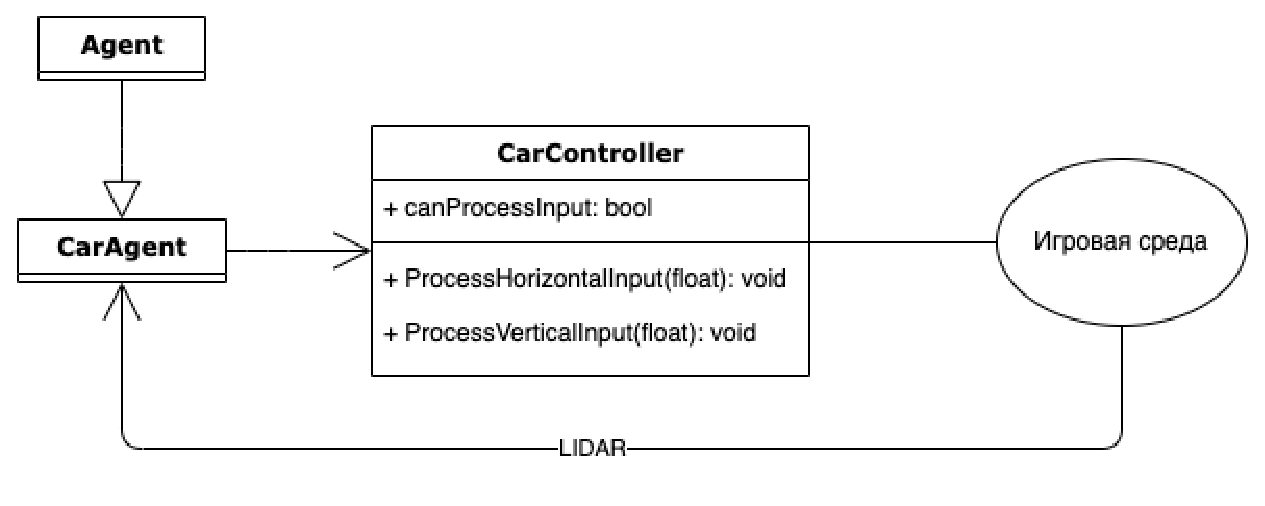
\includegraphics[width=0.75\textwidth]{images/diagram.drawio.eps}
	\caption{Схематическое изображение основной архитектуры проекта}
	\label{fig:diagram}
\end{figure}

Код реализации доступен в открытом репозитории на GitHub \cite{ratm}.

\subsection{Разработка нейросетевего метода тестирования игрового процесса}
В данной работе были рассмотрены подходы к тестированию игрового процесса по компактным представлениям состояний, основанные на следующих нейросетевых архитектурах: \textit{Proximal Policy Optimization} (\textit{PPO}) \cite{ppo} и \textit{Soft Actor-Critic} (\textit{SAC}) \cite{sac}.

В основе \textit{PPO} лежит консервативное обновление политики, ограничивающее соотношение между текущей и прежней политикой в диапазоне \([1-\varepsilon, 1+\varepsilon]\) (\(\varepsilon\) является гиперпараметром). Таким образом мы устраняем стимул, побуждающий нынешнюю политику слишком далеко отходить от предыдущей на каждой эпохе обучения. Функция потерь в архитектуре \textit{PPO} выглядит следующим образом:
\begin{equation}
	L^{\textit{CLIP}}(\theta) = \hat{E}_t[\min(r_t(\theta)\hat{A}_t, \textit{clip}(r_t(\theta), 1 - \varepsilon, 1 + \varepsilon)\hat{A}_t)],
\end{equation} где 
\begin{itemize}
	\item[--] \(\theta\) -- параметр политики;
	\item[--] \(r_t(\theta) = \frac{\pi_\theta(a_t \mid s_t)}{{\pi_\theta}_{old}(a_t \mid s_t)}\) -- отношение вероятностей при новой и старой политиках соответственно. Если \(r_t(\theta) > 1\), то действие \(a_t\) в состоянии среды \(s_t\) более вероятно в текущей политике, чем в предыдущей. В противном случае, если \(r_t(\theta) \in [0, 1]\), то данное действие в текущей политике будет менее вероятным;
	\item[--] \(\hat{E}_t\) обозначает математическое ожидание;
	\item[--] \(\hat{A}_t\) -- оценка <<преимущества>> (\textit{advantage}), которое агент получает при следовании политике \(\pi_\theta\). При \(\hat{A}_t > 0\) действие \(a_t\) в состоянии среды \(s_t\) дает лучший результат по сравнению с другими действиями в этом же состоянии.
\end{itemize}

Беря минимум, мы получаем нижнюю (пессимистическую) границу целевой функции, неограниченной диапазоном \([1-\varepsilon, 1+\varepsilon]\).

% TODO: картиночки!
В рамках эксперимента также была проведен поиск оптимальных значений гиперпараметров \(\varepsilon\) и \(\beta\), используемых в алгоритме. Результат оптимизации путем поиска по решетке приведен на рис.~\ref{fig:hyperopt}.

Этап тренировки агента был организован следующим образом:
\begin{itemize}
	\item[--] в начале каждой эпохи нейросетевой агент инициализировался случайным образом внутри параллелепипеда, ограничивающего игровое поле (Рисунок~\ref{fig:bounds}). Местом возникновения агента обязательно являлось дорожное полотно;
	\item[--] в течение 10 тысяч шагов (продолжительность эпохи подбиралась эмпирическим путем) агент исследовал игровую среду:
	\begin{itemize}
		\item[а)] в случае первичного нахождения локации вида \textit{out of bounds} агенту присуждалась награда в \(+1\) единицу. Этот вид бага зачастую является более критическим, и поэтому за его нахождение мы даем награду выше;
		\item[б)] в случае первичного нахождения локации вида с низким числом кадров в секунду агенту присуждалась награда в \(+0,1\) единицу. Здесь под <<низким числом>> понимается значение меньше 10 кадров/c, т.е. ниже медианного значения в условиях тренировки, округленного до целого числа. 
	\end{itemize}
	\item[--] по прошествии эпохи позиция и угол поворота агента сбрасывались и инициализировались заново, а веса модели обновлялись с использованием собранных наблюдений.
\end{itemize}

\begin{figure}
	\centering
	\includegraphics[width=0.75\textwidth]{images/bounds}
	\caption{Границы инициализации игрового агента (отмечены зеленым цветом)}
	\label{fig:bounds}
\end{figure}

\begin{figure}
	\centering
	\includegraphics[width=0.5\textwidth]{images/ppo\_hyperopt}
	\caption{Тепловая карта значений гиперпараметров \(\varepsilon\), \(\beta\) и суммарной награды на момент остановки обучения}
	\label{fig:hyperopt}
\end{figure}

В общем случае нейросетевой агент тренировался 100 эпох (или же, что то же самое, \(10^6\) шагов), и этап тренировки был повторен 10 раз для получения усредненных значений. Графики процесса обучения и функции потерь модели приведены на Рисунках~\ref{fig:training} и~\ref{fig:trainingValueLoss}. 

\begin{figure}
	\centering
	\includegraphics[width=0.75\textwidth]{images/output}
	\caption{Кривая обучения модели в 10 экспериментах. Для каждой эпохи приведены выборочное среднее и 95\%-й доверительный интервал}
	\label{fig:training}
\end{figure}

\begin{figure}
	\centering
	\includegraphics[width=0.75\textwidth]{images/output\_val\_loss}
	\caption{График функции потерь в 10 экспериментах. Для каждой эпохи приведены выборочное среднее и 95\%-й доверительный интервал}
	\label{fig:trainingValueLoss}
\end{figure}

\subsection{Оценка качества и апробация разработанных методов}
Результаты показывают, что получаемое агентом за эпоху среднее значение награды стабилизируется в процессе обучения. Также из Рисунка~\ref{fig:bugLocations} мы видим \(293\) точки на игровой карте, где в ходе одного из тренировочных запусков нейросетевой агент находил оба типа багов. Из карты также видно, что точки формируют <<проблемные>> кластеры: участки с низким числом кадров в секунду концентрируются вокруг травы и деревьев (свидетельство плохой оптимизации игровой зелени), а участки \textit{out of bounds} "--- рядом со зданиями (агент может выйти за пределы игровой среды, прижимаясь к основаниям зданий). Получаемая за найденные ошибки награда отражается в поведении полученного нейросетевого агента: после начала эпохи он стремится на скорости въехать в ближайшие препятствия, пытаясь найти проблемные участки среды.

\begin{figure}
	\centering
	\includegraphics[width=0.75\textwidth]{images/bug\_locations}
	\caption{Лучи исходят из точек на карте, где нейросетевой агент смог найти баги двух видов: \textit{out of bounds} (отмечены голубым) и участки с низким значением \textit{FPS} (отмечены красным)}
	\label{fig:bugLocations}
\end{figure}

%TODO: составить heatmap багов

\specialsection{Заключение}

Жизнь --- тлен.
%В ходе проделанной работы был продемонстрирован подход для автоматизированного тестирования игр путем исследования игровой среды при помощи алгоритма \textit{Proximal Policy Optimization}. На примере \textit{Race Against the Machine}, игры, разработанной в рамках научно-исследовательской работы, был создан <<бейзлайн>> для последующей выпускной квалификационной работы.
%
%В дальнейшем планируется расширение нейросетевего метода на алгоритм \textit{Soft Actor-Critic} (\textit{SAC}) \cite{haarnoja2018soft} и алгоритм семества \textit{Deep Q-Network} (например, \textit{Rainbow} \cite{hessel2017rainbow}), а также оптимизация гиперпараметров и сравнительный анализ полученных подходов. Также остается открытым вопрос нахождения ошибок в дизайне игры и проверка пользовательских сценариев. 


% Библиография в cpsconf стиле
% Аргумент {1} ниже включает переопределенный стиль с выравниванием слева
\begin{thebibliography}{1}
	
%%%%%%%%%%%%%%% Введение. Область применения
\bibitem{lopes2018games} Lopes~S., Magalh{\~a}es~P. et al. Games Used With Serious Purposes: A Systematic Review of Interventions in Patients With Cerebral Palsy // Frontiers in Psychology. 2018. Vol.~9. Art.~no~312205.
\bibitem{hassan2021serious} Hassan~A., Pinkwart~N., Shafi~M. Serious Games to Improve Social and Emotional Intelligence in Children With Autism // Entertainment Computing. 2021. Vol.~38. Art.~no~100417.
\bibitem{vahldick2020blocks} Vahldick~A., Farah~P.R. et al. A blocks-based serious game to support introductory computer programming in undergraduate education // Computers in Human Behavior Reports. 2020. Vol.~2. Art.~no~100037.
\bibitem{mayer2019computer} Mayer~R.E. Computer Games in Education // Annual review of psychology. 2019. Vol.~70. P.~531--549.
\bibitem{augustin2016we} Augustin~K., Thiebes~S. et al. Are We Playing Yet? A Review of Gamified Enterprise Systems // PACIS 2016 Proceedings. 2016.
\bibitem{politowski2021game} Politowski~C., Petrillo~F. et al. Game industry problems: An extensive analysis of the gray literature // Information and Software Technology. 2021. Vol.~134. Art.~no~106538.

%%%%%%%%%%%%%%% Введение. Обзорные статьи
\bibitem{xia2020recent} Xia~B., Ye~X., Abuassba~A.O.M. Recent Research on AI in Games // 2020 International Wireless Communications and Mobile Computing (IWCMC). 2020. P.~505--510.
\bibitem{santos2018computer} Santos~R.E.S., Magalh{\~a}es C.V.C. et al. Computer Games Are Serious Business and So Is Their Quality: Particularities of Software Testing in Game Development From the Perspective of Practitioners // Proceedings of the 12th ACM/IEEE International Symposium on Empirical Software Engineering and Measurement. 2018. P.~1--10.
\bibitem{truelove2021we} Truelove~A., de Almeida~E.S., Ahmed~I. We'll Fix It in Post: What Do Bug Fixes in Video Game Update Notes Tell Us? // 2021 IEEE/ACM 43rd International Conference on Software Engineering (ICSE). IEEE, 2021. P.~736--747.
\bibitem{murphy2014cowboys} Murphy-Hill~E., Zimmermann~T., Nagappan~N. Cowboys, ankle sprains, and keepers of quality: How is video game development different from software development? // Proceedings of the 36th International Conference on Software Engineering. 2014. P.~1--11.

%%%%%%%%%%%%%%% Обзор нейросетевых подходов тестирования игрового процесса
\bibitem{aleem2016critical} Aleem~S., Capretz~L.F., Ahmed~F. Critical success factors to improve the game development process from a developer’s perspective // Journal of computer science and technology. 2016. Vol.~31. P.~925--950.
%%%%%%%%%%%%%%% Ссылки на библиотеки

%%%%%%%%%%%%%%% Конец ссылок на библиотеки
\bibitem{sutton2018reinforcement} Sutton~R.S., Barto~A.G. Reinforcement Learning: An Introduction. MIT press, 2018.
\bibitem{politowski2021survey} Politowski~C., Petrillo~F., Gu{\'e}h{\'e}neuc~Y.\:G. A Survey of Video Game Testing // 2021 IEEE/ACM International Conference on Automation of Software Test (AST). IEEE, 2021. P.~90--99.
\bibitem{mnih2013playing} Mnih~V., Kavukcuoglu~K. et al. Playing Atari with Deep Reinforcement Learning // arXiv preprint arXiv:1312.5602. 2013.
\bibitem{borovikov2019winning} Borovikov~I., Zhao~Y. et al. Winning Isn’t Everything: Training Agents to Playtest Modern Games // AAAI Workshop on Reinforcement Learning in Games. 2019.
\bibitem{silver2017mastering} Silver~D., Hubert~T. et al. Mastering Chess and Shogi by Self-Play With a General Reinforcement Learning Algorithm // arXiv preprint arXiv:1712.01815. 2017.
\bibitem{bergdahl2020augmenting} Bergdahl~J., Gordillo~C. et al. Augmenting Automated Game Testing With Deep Reinforcement Learning // 2020 IEEE Conference on Games (CoG). IEEE, 2020. P.~600--603.
\bibitem{henderson2018deep} Henderson~P., Islam~R. et al. Deep Reinforcement Learning That Matters // Proceedings of the AAAI Conference on Artificial Intelligence. 2018. Vol.~32. \textnumero.~1.
\bibitem{tufano2022using} Tufano~R., Scalabrino~S. et al. Using reinforcement learning for load testing of video games // Proceedings of the 44th International Conference on Software Engineering. 2022. P.~2303--2314.

%%%%%%%%%%%%%%% Разработка эмуляционной игровой среды и методов тестирования
\bibitem{ratm} RATM [Электронный ресурс] // GitHub. \url{URL: https://github.com/MicAPic/RATM} (дата обращения: 24.03.23).
\bibitem{ppo} Proximal Policy Optimization [Электронный ресурс] // OpenAI. \url{URL: https://openai.com/research/openai-baselines-ppo} (дата обращения: 24.03.23).
\bibitem{sac} Haarnoja~T., Zhou~A. et al. Soft Actor-Critic: Off-Policy Maximum Entropy Deep Reinforcement Learning With a Stochastic Actor // International Conference on Machine Learning. PMLR, 2018. P.~1861--1870.

\end{thebibliography}
\end{document}